% ===========================================================================
% Section 11. Robustness and validation
% Numbers: paper/results/robustness.json (scripts/paper/fig_robustness.R) and
% paper/results/network_robustness.json (scripts/paper/fig_network_robustness.R); final rerun of
% 2026-10-12. Further detail (vintages, weight draws, curvature, imputation, rankability,
% leave-one-out and effective importance, data choices, vertical complementarities with the
% appendix sensitivity table tab:robustness_vertical): Online Appendix oa:robustness
% (sections/oa_robustness.tex).
% ===========================================================================
\section{Robustness and validation}
\label{sec:robustness}

We vary one element of the construction at a time, holding the others at the final configuration,
and ask how far the results depend on choices rather than data
\citep{saisana2005uncertainty,oecd2008handbook,saltelli2008global}. For the pillars the comparison
that matters is the ranking of countries within a technology--stage pair, so the main statistic is
the within-pair Spearman correlation with the baseline, summarised across pairs and computed over
the baseline's rankable cells: 4{,}163 of 6{,}232 scored cells in the 30 headline $\ES$ pairs and
4{,}301 of 7{,}131 in the 33 $\EO$ pairs. Every variant is recomputed from stored inputs with the
pipeline's own builders, which reproduce the published indices at the baseline settings. Online
Appendix~\ref{oa:robustness} gives the details and further tables.

% ---------------------------------------------------------------------------
\subsection{The pillars}
\label{subsec:robust_pillars}

Within-pair rankings are almost insensitive to the category weights and to the curvature of the
S-curve (Figure~\ref{fig:robustness_variants}). Over 1{,}000 Dirichlet draws centred on the
configured weights (coefficient of variation 0.3 for a category of average weight), the median
within-pair correlation is 0.997 in $\ES$ and 0.988 in $\EO$, and equal weights give 1.000.
Re-curving every component to $\gamma=0.25$, 1 (the plain percent rank) or 2 gives medians between
0.964 and 0.997 in $\ES$ and between 0.965 and 0.992 in $\EO$, the lowest at $\gamma=2$. Much of
this stability is mechanical: all scored countries of a pair observe the same categories, so a
category that is constant within the pair shifts every country alike
(equation~\eqref{eq:affine_constant}), and the median pair has only three varying categories in
$\ES$ and four in $\EO$. A high average can also hide wide rank bands for individual members
(Online Appendix~\ref{oa:robustness}).

The imputation rule matters more. Without the global-average imputation $\ES$ is unchanged in the
median pair (1.00) and $\EO$ nearly so (0.97), but the pooled $\EO$ correlation is 0.85 and the
minimum 0.29; filling gaps with zeros lowers the $\EO$ median to 0.77. Outside the economies that the
narrow sources cover, $\EO$ rankings depend on how gaps are filled, which is why the rankability rule
withholds cells whose index rests mostly on imputed components. Its threshold is itself
consequential: at $\tau=0.3$ the Strategic Index shrinks from 3{,}154 cells for 174 countries to
1{,}577 cells for 107, and at $\tau=0.7$ it grows to 5{,}156 cells for 194. The 2020 and 2025
vintages, which re-derive only the time-varying sources (about a third of the average cell's
weight), give median within-pair correlations of 0.99 in $\ES$ and 0.87 in $\EO$. Leaving out one
category confirms that nominal weights and effective importance diverge
\citep{paruolo2013ratings,becker2017weights}: Technology Demand, the largest nominal $\EO$ weight,
barely moves the median ranking, while Foreign Dependency, Cost Competitiveness and Trade carry most
of it.

\begin{figure}[tbp]
  \centering
  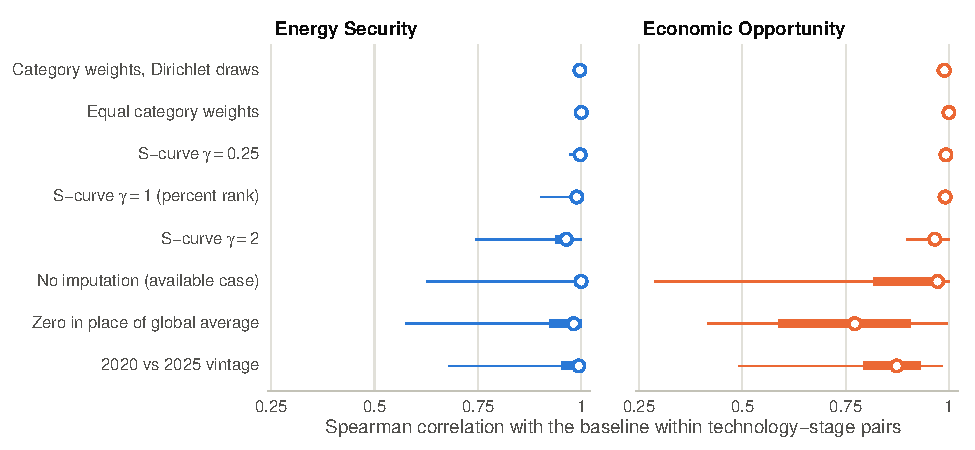
\includegraphics[width=\textwidth]{robustness_variants}
  \caption{Stability of within-pair country rankings under alternative constructions of the
  pillars. Each row is one variant; for each technology--stage pair the Spearman rank correlation
  across countries between the baseline pillar and the variant is computed over the baseline's
  rankable cells, and the row summarises these correlations across pairs: open circle, median;
  thick bar, interquartile range; thin line, minimum to maximum. For the Dirichlet weight draws the
  per-pair value is the median over 1{,}000 draws. The S-curve rows rebuild both pillars from the
  theme tables with every component re-curved to $\gamma=0.25$, 1 or 2 (baseline 0.5). ``No
  imputation'' removes every global-average rule, so uncovered countries drop the component;
  ``Zero'' fills them with 0. The last row compares the 2020 and 2025 vintages. Sample: 30 $\ES$
  pairs (4{,}163 rankable cells) and 33 $\EO$ pairs (4{,}301). Source: \texttt{index\_outputs.rds},
  theme tables and vintages of the final run; \texttt{scripts/paper/fig\_robustness.R}.}
  \label{fig:robustness_variants}
\end{figure}

% ---------------------------------------------------------------------------
\subsection{The Strategic Index and the allied picks}
\label{subsec:robust_si}

The ordering of a country's sectors is robust; its single top sector is not. Under 1{,}000 Dirichlet
draws of the five weights of equation~\eqref{eq:si}, the median within-country Spearman correlation
is 0.96 (0.88 to 0.99), but a member keeps its allied pick in 73 per cent of the draws on average,
16 of the 57 members in at least 90 per cent and 10 in fewer than half
(Figure~\ref{fig:robustness_si}). Retention follows the pick's margin over the runner-up (Spearman
correlation 0.84), and the margins are small: a median of 0.015, below 0.005 for 10 members and
below 0.01 for 21, smallest for Luxembourg (0.0005) and Indonesia (0.0007). Electric Grid and Nuclear
Midstream picks rest on the finest margins (medians 0.003 and 0.007, against 0.014 for Batteries
Midstream). The Nuclear Midstream picks of Costa Rica, the Dominican Republic, Guatemala and Namibia
have wide margins for a reason other than capability, and not because of a floor in the security
pillar: each may pick among only four sectors, the Midstream stages of nuclear, oil, gas and coal
(Namibia also Nuclear Upstream), Midstream nuclear security is compressed around its median, and the
technology greenhouse-gas weight favours nuclear (0.999, against 0.42 for gas, 0.02 for coal and 0
for oil); without the sector priors the Dominican Republic, Guatemala and Namibia move to Oil
Midstream.

Table~\ref{tab:robustness_picks} reports discrete variants. Reading security as strength rather
than need is the most consequential: the pooled Spearman correlation with the baseline is 0.33 and
only 5 of the 57 picks survive. Without the sector priors 31 picks survive, with all terms ranked
within country 20, without the policy term 30 and with equal weights 39. Switching the endowment
screen off changes 41 picks, raising Upstream picks from 14 to 47: a country without uranium scores
zero on the reserve and production terms, sits near the floor of the security pillar (86 of 174
countries share one $\ES$ value in Nuclear Upstream) and so shows a high need. The screen is a rule
of eligibility, not part of the index, and without it the Upstream picks would largely reflect that
floor. Tightening the screen to require recorded production, rather than any recorded
reserves, removes all eight Nuclear Upstream picks, whose holders have small identified resources
and no mine production, and the two Wind Upstream picks: nine members change pick and Gabon is left
without an eligible sector. Two variants address the implicit sector priors of
Section~\ref{subsec:si_definition}. Removing the cell-constant inputs from the pillar levels keeps
the within-member ordering (median Spearman correlation 0.95) but only 29 of the 57 picks, and 23 picks
then fall on Electric Grid Midstream; entering opportunity and need as within-pair ranks keeps 27
picks (median within-member correlation 0.80). The basis of the Policy index matters for its values more than for the picks: for the 65
countries with both components, the within-country correlation between policy on IEA PAMS alone and
on the composite has a median of 0.48 (interquartile range 0.41 to 0.57), yet IEA PAMS alone keeps
45 picks, and requiring both components keeps the 46 CAT-rated members' picks exactly while removing
the 11 scored on IEA PAMS alone. Adding back the October 2026 NIPO component (77 jurisdictions)
keeps only 34 picks, shifting them from Batteries Midstream (27 to 15) towards Nuclear Upstream (8 to
14).

The picks also rest on the trade data. Setting the EIA-filled fossil production to zero changes no
pick and removing the new Upstream trade baskets changes four, but dropping the Trade category keeps
29 of the 54 members that still have a pick, Trade on the Atlas basis 49, and the 2025 and 2020
vintages 48 and 44. The recorded history agrees: before the energy-trade file was completed,
Electric Grid Midstream was the pick of 17 and Batteries Midstream of 11 of the 45 members then with
a pick, against 4 and 27 of 57 in the final build. The allied pick is an informative but fragile summary, stable to the fill rules and
basket additions of the final revision and sensitive to how trade is measured.

\begin{figure}[tbp]
  \centering
  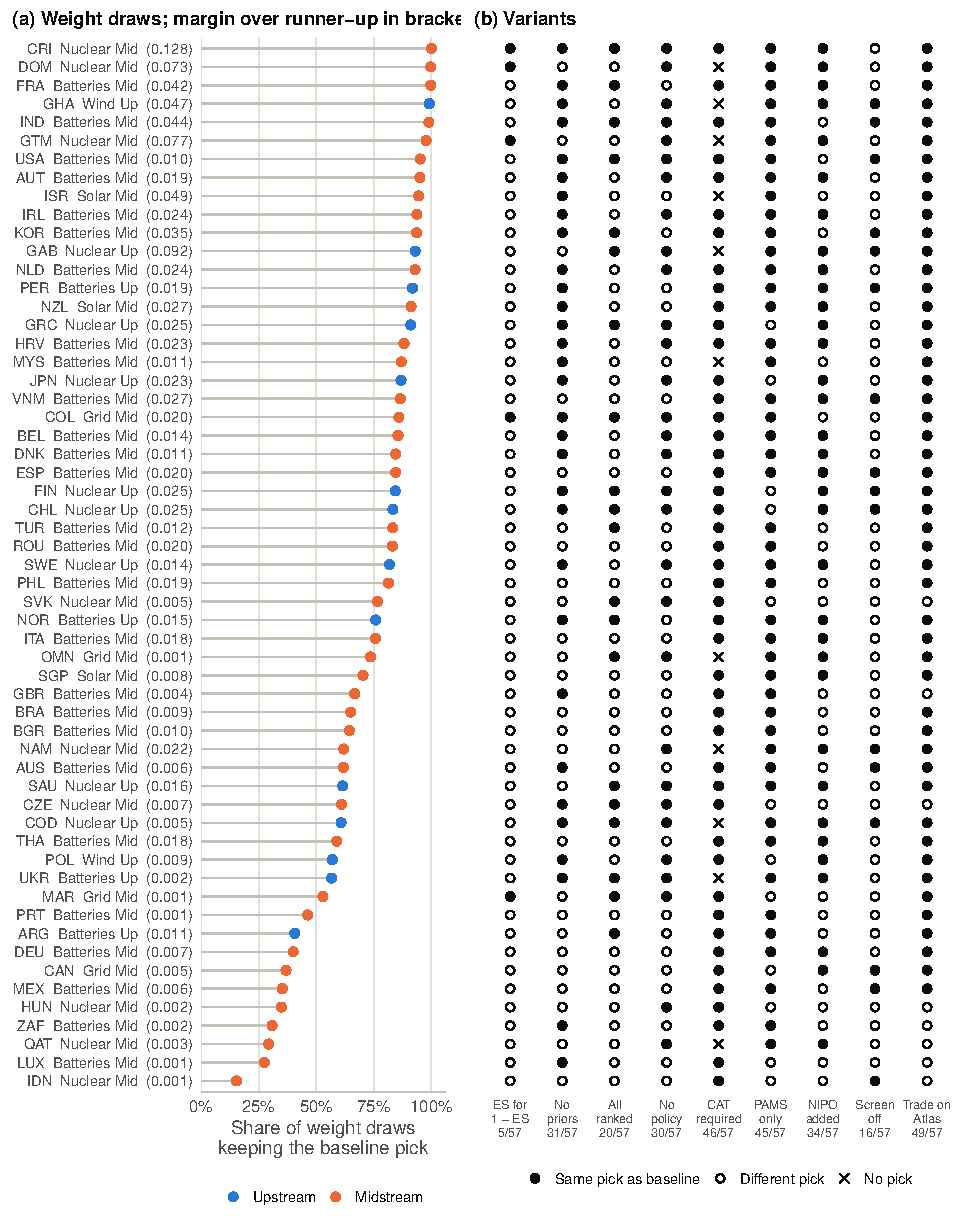
\includegraphics[width=\textwidth,height=0.70\textheight,keepaspectratio]{robustness_si}
  \caption{Robustness of the allied picks. Each row is a coalition member, its baseline pick (the
  eligible Upstream or Midstream sector with the highest Strategic Index) and, in brackets, the
  margin over its second eligible sector. Panel~(a): share of 1{,}000 Dirichlet draws of the five
  Strategic Index weights, centred on $(0.2,0.3,0.3,0.1,0.1)$ with concentration 43.4, under which
  the pick is unchanged; colour gives the stage of the pick. Panel~(b): filled circle, pick
  unchanged under the variant; open circle, changed; cross, no pick. Variants: security in place of
  need; no stage and technology priors; $\EO$ and $1-\ES$ S-curved within country; no policy term;
  both Policy components required; IEA PAMS only; the October 2026 NIPO component added back; the
  endowment screen off; Trade on the Atlas basis. Sample: 3{,}154 Strategic Index cells of 174
  countries; 57 members, all with a baseline pick. Source: \texttt{index\_outputs.rds},
  \texttt{policy\_component\_tbl}, the October 2026 NIPO component;
  \texttt{scripts/paper/fig\_robustness.R}.}
  \label{fig:robustness_si}
\end{figure}

% Generated by scripts/paper/fig_robustness.R; do not edit by hand.
\begin{table}[tbp]
  \centering
  \begin{threeparttable}
  \caption{Allied picks by sector under the baseline and the variants of the Strategic Index}
  \label{tab:robustness_picks}
  \footnotesize
  \setlength{\tabcolsep}{4pt}
  \begin{tabular}{lrrrrrrrrr}
    \toprule
    \multicolumn{10}{l}{\emph{Panel A. Specification and Policy index}}\\
    Sector & \makecell{Base-\\line} & \makecell{$\ES$ for\\$1-\ES$} & \makecell{No\\priors} & \makecell{All\\ranked} & \makecell{No\\policy} & \makecell{Equal\\weights} & \makecell{CAT\\required} & \makecell{PAMS\\only} & \makecell{NIPO\\added} \\
    \midrule
    Nuclear Upstream & 8 & 2 & 14 & 13 & 20 & 1 & 6 & 4 & 14 \\
    Batteries Upstream & 4 & 1 & 3 & 4 & 2 & 2 & 3 & 4 & 6 \\
    Wind Upstream & 2 & 0 & 2 & 0 & 3 & 1 & 1 & 1 & 3 \\
    Coal Upstream & 0 & 0 & 1 & 0 & 0 & 0 & 0 & 0 & 0 \\
    Electric Grid Upstream & 0 & 3 & 1 & 1 & 1 & 0 & 0 & 0 & 0 \\
    Electric Vehicles Upstream & 0 & 0 & 1 & 0 & 0 & 0 & 0 & 0 & 0 \\
    Gas Upstream & 0 & 1 & 0 & 0 & 0 & 0 & 0 & 0 & 0 \\
    Oil Upstream & 0 & 2 & 3 & 0 & 0 & 0 & 0 & 0 & 0 \\
    Solar Upstream & 0 & 0 & 2 & 4 & 1 & 0 & 0 & 0 & 2 \\
    Batteries Midstream & 27 & 0 & 15 & 5 & 8 & 30 & 26 & 34 & 15 \\
    Nuclear Midstream & 9 & 28 & 2 & 8 & 9 & 8 & 5 & 5 & 7 \\
    Electric Grid Midstream & 4 & 7 & 1 & 15 & 13 & 4 & 3 & 3 & 5 \\
    Solar Midstream & 3 & 2 & 2 & 1 & 0 & 9 & 2 & 6 & 4 \\
    Electric Vehicles Midstream & 0 & 0 & 0 & 0 & 0 & 0 & 0 & 0 & 1 \\
    Gas Midstream & 0 & 10 & 0 & 0 & 0 & 0 & 0 & 0 & 0 \\
    Oil Midstream & 0 & 1 & 10 & 6 & 0 & 0 & 0 & 0 & 0 \\
    Wind Midstream & 0 & 0 & 0 & 0 & 0 & 2 & 0 & 0 & 0 \\
    \midrule
    Members with a pick & 57 & 57 & 57 & 57 & 57 & 57 & 46 & 57 & 57 \\
    Same pick as baseline & 57 & 5 & 31 & 20 & 30 & 39 & 46 & 45 & 34 \\
    \addlinespace
    \midrule
    \multicolumn{10}{l}{\emph{Panel B. Data: endowment screen, final data choices, trade and reserves inputs, vintage}}\\
    Sector & \makecell{Base-\\line} & \makecell{Screen\\off} & \makecell{Zero for\\EIA} & \makecell{No new\\baskets} & \makecell{Trade on\\Atlas} & \makecell{No\\Trade} & \makecell{No\\Reserves} & \makecell{2025\\vintage} & \makecell{2020\\vintage} \\
    \midrule
    Nuclear Upstream & 8 & 17 & 8 & 11 & 8 & 9 & 14 & 9 & 8 \\
    Batteries Upstream & 4 & 12 & 4 & 4 & 4 & 1 & 1 & 4 & 5 \\
    Wind Upstream & 2 & 5 & 2 & 1 & 2 & 1 & 2 & 2 & 1 \\
    Electric Grid Upstream & 0 & 1 & 0 & 0 & 0 & 0 & 0 & 0 & 0 \\
    Solar Upstream & 0 & 12 & 0 & 0 & 0 & 0 & 0 & 0 & 0 \\
    Batteries Midstream & 27 & 7 & 27 & 25 & 26 & 13 & 24 & 25 & 23 \\
    Nuclear Midstream & 9 & 2 & 9 & 9 & 4 & 0 & 8 & 4 & 4 \\
    Electric Grid Midstream & 4 & 1 & 4 & 4 & 5 & 10 & 4 & 5 & 11 \\
    Solar Midstream & 3 & 0 & 3 & 3 & 7 & 19 & 4 & 7 & 5 \\
    Electric Vehicles Midstream & 0 & 0 & 0 & 0 & 0 & 1 & 0 & 0 & 0 \\
    Gas Midstream & 0 & 0 & 0 & 0 & 1 & 0 & 0 & 1 & 0 \\
    \midrule
    Members with a pick & 57 & 57 & 57 & 57 & 57 & 54 & 57 & 57 & 57 \\
    Same pick as baseline & 57 & 16 & 57 & 53 & 49 & 29 & 50 & 48 & 44 \\
    \bottomrule
  \end{tabular}
  \begin{tablenotes}[flushleft]\scriptsize
    \item \emph{Notes:} Number of coalition members whose allied pick, the Upstream or Midstream sector (excluding Geothermal and Green Hydrogen, and Upstream cells without a recorded resource base) with the highest Strategic Index, falls in each sector. All 57 members have a pick in the baseline. Panel A: $\ES$ for $1-\ES$, security in place of need; No priors, without the stage and technology terms; All ranked, $\EO$ and $1-\ES$ S-curved within country; No policy, without the policy term; Equal weights, 0.2 on each term; CAT required, both Policy components required (\texttt{OPSI\_POLICY\_REQUIRE\_ALL=1}), which leaves 65 countries with a Policy index and 46 members with a pick; PAMS only, CAT dropped for every country; NIPO added, the October 2026 NIPO component (GTA NIPO as of 5 October 2026) re-enters the Policy index with weight 4 (IEA PAMS 3, CAT 2), IEA PAMS still required, for its 77 policy-eligible jurisdictions. Panel B: Screen off, every Upstream cell eligible, including the 669 of 998 scored Upstream cells without recorded reserves or production; Zero for EIA, the oil, gas and coal production that the Energy Institute does not report set to zero instead of the EIA value (the rule until 11 October 2026); No new baskets, the Trade category removed from Electric Vehicles, Wind, Nuclear and Solar Upstream, whose trade baskets were added on 11 October 2026; Trade on Atlas, the Trade category of both pillars replaced by its Atlas-based counterpart of the 2025 vintage; No Trade, No Reserves, the category dropped from the pillars that score it and the remaining categories renormalised; 2025 and 2020 vintage, both pillars taken from the vintage builds, in which only the time-varying sources differ. The Policy index is the headline one in Panel B. Source: \texttt{index\_outputs.rds}, \texttt{data/processed/vintages}; \texttt{scripts/paper/fig\_robustness.R}.
  \end{tablenotes}
  \end{threeparttable}
\end{table}


% ---------------------------------------------------------------------------
\subsection{Vertical complementarities}
\label{subsec:robust_vertical}

The pillars score each stage separately, although shocks propagate along input--output links
\citep{acemoglu2012network,carvalho2021supply} and capabilities in one activity ease entry into
related ones \citep{hidalgo2007product}. A companion study tested whether a stage's $\EO$ should
reward capability in the adjacent stage and its $\ES$ the security of its inputs. On the Atlas panel
of 172 economies (1995--2023), with country--year and technology--year fixed effects, adjacent-stage
capability is associated with a stage's market-share growth and entry into comparative advantage
\citep{balassa1965trade} across countries, but the association is concentrated in fossil fuels and
nuclear, close to zero for the clean-technology chains, zero within country--technology cells, and
of no help out of sample. A sourcing-weighted input-security measure reflects mostly alignment, its
post-2022 shift is driven by Russia, and it did not predict the import shortfalls of 2021--22, whereas
the concentration of sourcing did. At the weights the evidence supports, an adjacent-stage $\EO$
term moves one pick and an input-security $\ES$ term moves ten, no more than a placebo with permuted
scores (Online Appendix~\ref{oa:robustness}). We therefore keep the stages uncoupled and leave to
future work plant-level co-location from the CM-FDI and BNEF project data, input shares weighted by
input--output coefficients, a test of sourcing concentration on the 2023 export controls on graphite
and gallium, and a co-location term in the network design.

% ---------------------------------------------------------------------------
\subsection{The partnership index}
\label{subsec:robust_psi}

The headline PSI averages the dyadic index over the 31 core members' viewpoints. The full-coalition
view (57 reporters) gives nearly the same ranking (Spearman correlation 0.98 over 192 partners, 13 of
the top 15 in common), although China moves from 44th to 9th; the world view (218 reporters) differs
more (0.88, 10 of the top 15, median absolute rank change 17). The viewpoint is a choice of whose
interests the index represents (Figure~\ref{fig:robustness_psi_views}). Without the CM-FDI parts of
friendshore, in the integration study on the inputs of 11 October 2026, the core PSI is practically
unchanged (Spearman correlation 0.9998, largest rank change five places, same top 15).

Two further sensitivities concern Friendshore. Scoring an absent outward-investment record at the
lowest rank rather than dropping it from the available-case mean leaves the core PSI almost
unchanged (Spearman correlation 0.994, 14 of the top 15 in common, largest rank change 34 places,
China from 44th to 37th), although it reorders the top suppliers of individual reporters
(Section~\ref{sec:bilateral}). The discretisation of alignment matters more. With continuous
alignment, $p_i=s_i$ so that $A_{ij}=s_is_j+(1-s_i)(1-s_j)$, the Spearman correlation with the
headline is 0.904, 12 of the top 15 are shared, the median partner moves 13.5 places and China
rises from 44th to 9th; with tercile blocs (cuts at $s=0.164$ and 0.305, 65 economies in each outer
bloc) the correlation is 0.952, 14 of the top 15 are shared and China ranks 40th. The quartile
cuts thus hold China down mainly through the step from a continuous to a three-valued alignment,
less through where the cuts fall.

\begin{figure}[tbp]
  \centering
  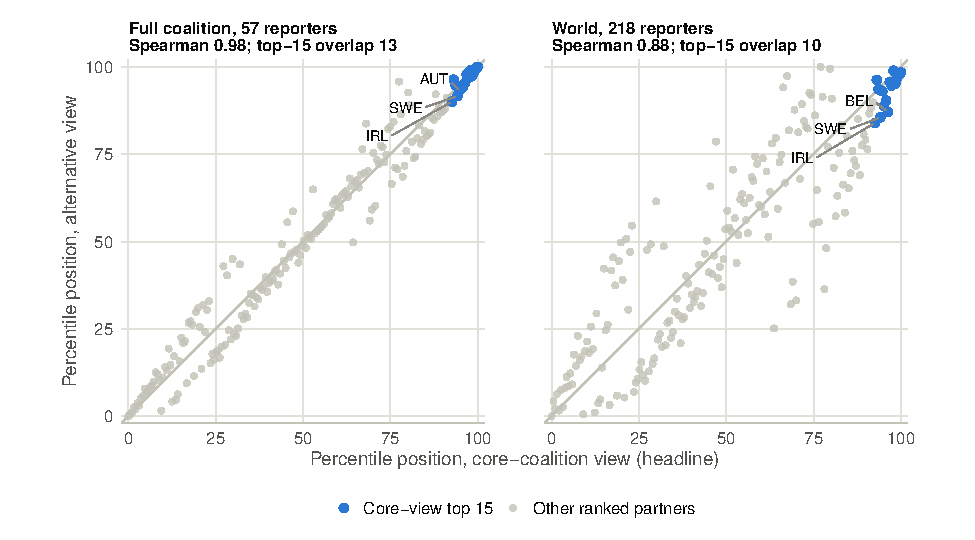
\includegraphics[width=\textwidth]{robustness_psi_views}
  \caption{The partnership index from three viewpoints. Each point is a partner ranked in both
  views ($\tau=0.5$), placed by its percentile position in the core-coalition view, the headline
  average over the 31 core members' ratings (horizontal), and in an alternative view (vertical):
  left, the full coalition of 57 reporters; right, the world of 218 reporters. Blue marks the top 15
  of the core view; the labelled points are the three of them with the lowest position in the
  alternative view. Panel titles give the Spearman correlation with the core view and the overlap of
  the top 15. Source: \texttt{psi\_tbl.rds}, \texttt{psi\_full\_coalition\_tbl.rds},
  \texttt{psi\_world\_tbl.rds}; \texttt{scripts/paper/fig\_robustness.R}.}
  \label{fig:robustness_psi_views}
\end{figure}

% ---------------------------------------------------------------------------
\subsection{The network design}
\label{subsec:robust_network}

Figure~\ref{fig:network_robustness} and Table~\ref{tab:network_robustness} re-solve the design of
Section~\ref{sec:network} with one setting changed, on inputs assembled as in production (the re-run
of the production configuration reproduces it to $5\times10^{-16}$). Each variant is compared with
the production design stage by stage through the Jaccard overlap of the producer sets and the share
of production reassigned, $\tfrac12\sum_p|x^{\mathrm{alt}}_{p,ts}-x_{p,ts}|$. The neighbouring values
of $\lambda$ leave the design almost unchanged: at 0.77, 21 of the 22 producer sets are identical
and 0.5 per cent of production is reassigned in the mean stage; at 0.79, 19 and 1.1 per cent. The
calibration is knife-edge in its number, not in what it selects. Demand matters little, since it
enters the choice of producers only through the edges and redundancy constraints and is
rank-compressed (size only: 3.4 per cent reassigned). The edge weight matters more ($w_E=0$ and 1
reassign 8.4 and 10.8 per cent), and the portfolio caps most: without them 18.5 per cent of
production is reassigned in the mean stage, 46.5 per cent in Electric Grid Upstream. Solved greedily
with the caps, the design is more concentrated (median index 0.160, above the calibration target) and
scores 2.5 per cent lower. These tests concern the stability of the design to its specification, not
its robustness to shocks, which the program does not model beyond the redundancy floor.

\begin{figure}[tbp]
  \centering
  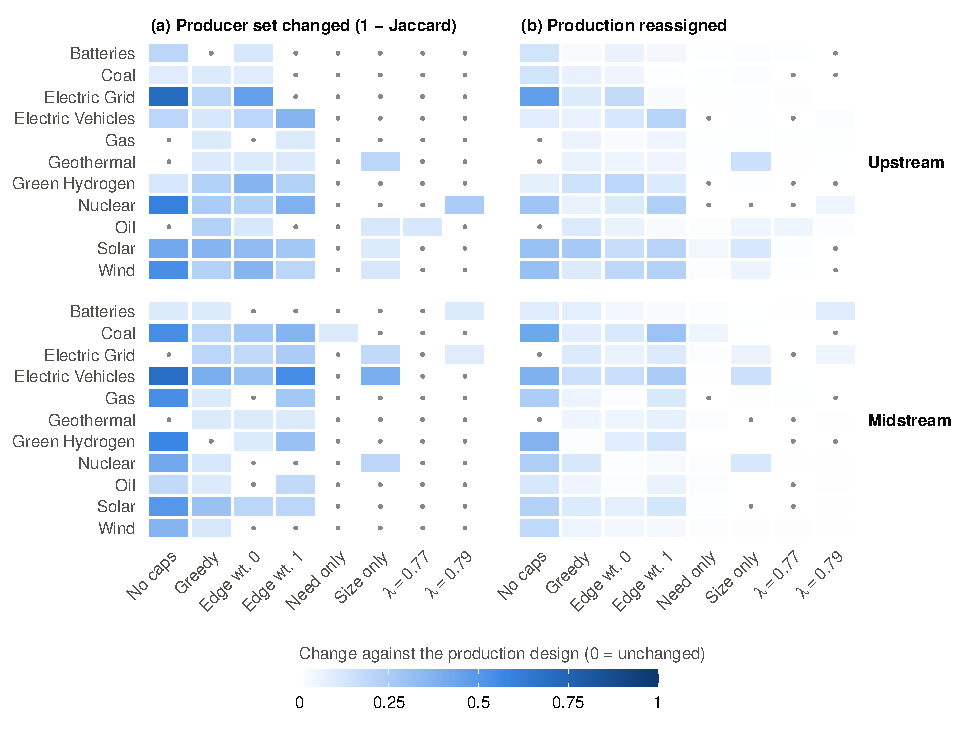
\includegraphics[width=\textwidth]{network_robustness}
  \caption{Robustness of the network design, by stage and variant. Each column re-solves the 22
  Upstream and Midstream stage programs on the 37 nodes with one setting changed: no portfolio
  caps; the greedy heuristic instead of the MILP (caps on); edge weight $w_E=0$ or 1 instead of
  0.5; demand from need only or size only; and $\lambda=0.77$ or 0.79 instead of 0.78.
  Panel~(a): one minus the Jaccard overlap $|A\cap B|/|A\cup B|$ of the stage's producer sets in the
  variant and the production design. Panel~(b): share of the stage's production assigned to
  different nodes, $\tfrac12\sum_p|x^{\mathrm{alt}}_{p,ts}-x_{p,ts}|$. Both are 0 when the stage is
  unchanged (dot) and 1 when the producer sets are disjoint. Source:
  \texttt{scripts/paper/fig\_network\_robustness.R}, on the inputs of the final rerun of 12 October
  2026.}
  \label{fig:network_robustness}
\end{figure}

% Generated by scripts/paper/fig_network_robustness.R
\begin{table}[htbp]
\centering
\begin{threeparttable}
\caption{Robustness of the network design to one setting at a time}
\label{tab:network_robustness}
\footnotesize
\begin{tabular}{@{}l r r r r r r r r@{}}
\toprule
 & \multicolumn{4}{c}{Against the production design} & \multicolumn{4}{c}{Design of the variant} \\
\cmidrule(lr){2-5}\cmidrule(l){6-9}
Variant & Jaccard & Min. & \makecell[r]{Identical\\stages} & \makecell[r]{Re-\\assigned} & \makecell[r]{Median\\$\HHI^{\mathrm{D}}$} & \makecell[r]{Pro-\\ducers} & \makecell[r]{Max.\\share} & \makecell[r]{MILP\\stages} \\
\midrule
Production design & -- & -- & -- & -- & 0.152 & 9 & 0.325 & 22 \\
\addlinespace
No portfolio caps & 0.692 & 0.294 & 5 & 0.185 & 0.139 &   10 & 0.312 & 22 \\
Greedy heuristic & 0.836 & 0.600 & 2 & 0.086 & 0.160 &    9 & 0.346 & 0 \\
Edge weight $w_E=0$ & 0.840 & 0.538 & 6 & 0.084 & 0.146 &    9 & 0.295 & 22 \\
Edge weight $w_E=1$ & 0.825 & 0.455 & 7 & 0.108 & 0.157 &    9 & 0.355 & 22 \\
Demand from need only & 0.995 & 0.900 & 21 & 0.010 & 0.154 &    9 & 0.325 & 22 \\
Demand from size only & 0.941 & 0.600 & 15 & 0.034 & 0.159 &    9 & 0.325 & 22 \\
$\lambda=0.77$ & 0.995 & 0.889 & 21 & 0.005 & 0.156 &    9 & 0.325 & 22 \\
$\lambda=0.79$ & 0.980 & 0.750 & 19 & 0.011 & 0.149 &    9 & 0.325 & 22 \\
\bottomrule
\end{tabular}
\begin{tablenotes}[flushleft]\footnotesize
\item \emph{Notes:} Production design: $\lambda=0.78$, GDP-log portfolio caps, edge weight $w_E=0.5$, demand from the equal mix of need and size, MILP. Each other row re-solves the 22 Upstream and Midstream stage programs on the 37 network nodes with one setting of the production design changed. Jaccard: mean across stages of the Jaccard overlap $|A\cap B|/|A\cup B|$ of the stage's producer set with that of the production design; Min.: its smallest value; Identical stages: stages with the same producer set. Reassigned: mean across stages of the share of production assigned to different nodes, $\tfrac12\sum_p|x^{\mathrm{alt}}_{p,ts}-x_{p,ts}|$ (0 when the shares are unchanged, 1 when the producer sets are disjoint). Median $\HHI^{\mathrm{D}}$: median across stages of the Herfindahl index of designed shares. Producers: median number of producers per stage. Max. share: largest designed share in any stage. MILP stages: stages solved by the MILP (the greedy row solves all stages heuristically). Source: \texttt{scripts/paper/fig\_network\_robustness.R}.
\end{tablenotes}
\end{threeparttable}
\end{table}


% ---------------------------------------------------------------------------
\subsection{What the analysis does and does not establish}
\label{subsec:robust_limits}

Within the ranges explored, the within-pair rankings of $\ES$ are robust to weights, curvature and,
over rankable cells, imputation, and those of $\EO$ to weights and curvature but not to imputation.
The Strategic Index orders a country's sectors stably, while the allied pick, a single arg max, is
robust only where its margin is large. There is no external validation: no outcome series of
realised disruptions or later export growth exists against which to test the pillars, and stability
shows that the rankings are determined by the data and the construction, not that they are right
\citep{ravallion2012mashup}. The perturbations are local and one at a time, and several data choices
are not varied: the exclusion of electricity from the grid basket and of Hong Kong's re-exports from
the export measures, the treatment of non-reporting economies through mirror declarations, the rank
compression of the EU's demand weight, the regional IEA 2035 manufacturing shares that every EU
member inherits in the foreign-dependency and market-share variables, and the zero counted for
unquantified USGS holdings. In the network design, the self-edge weight (the median observed edge),
the dual-sourcing rule (at least two suppliers, each at least 10 percent of demand) and the share
bound of 0.40 are not varied, and they shape the designed flows: self-supply is rare and most
consumer--stage pairs draw on exactly two suppliers by construction.
